\documentclass[a4paper,12pt,bibliography=totocnumbered]{report}
\usepackage[left=2.54cm, right=2.54cm, top=2.54cm, bottom=2.54cm]{geometry}%newly changes 2 to 2.54 
\usepackage{graphicx}
\usepackage{enumitem}
\usepackage{etoolbox}
\usepackage{tocloft}
\usepackage{float}%newly added
\floatstyle{plaintop}%newly added
\restylefloat{table}%newly added
\usepackage[titletoc]{appendix}%newly added
%\setlength{\cftbeforetoctitleskip}{em}
\renewcommand{\cftdot}{}%newly added
\renewcommand{\contentsname}{\hfill \Large CONTENTS} 
\renewcommand\cftaftertoctitle{\hfill\llap{\bfseries Page No.}}
\renewcommand{\cftlottitlefont}{\hspace*{\fill}\large\bfseries}
\renewcommand{\cftafterlottitle}{\hspace*{\fill} \linebreak \linebreak {\bfseries Table No.} \hfill {\bfseries Title} \hfill {\bfseries Page No.}}
\renewcommand{\cftloftitlefont}{\hspace*{\fill}\large\bfseries}
\renewcommand{\cftafterloftitle}{\hspace*{\fill} \linebreak \linebreak {\bfseries Figure No.} \hfill {\bfseries Title} \hfill {\bfseries Page No.}}
\graphicspath{{./images/}}
%\usepackage{tocbibind} %newly added
\usepackage{booktabs}
\usepackage{float}
\usepackage{caption}
\captionsetup{font=footnotesize}
\usepackage{nomencl}%[intoc] removed newly added
\makenomenclature
\renewcommand{\nomname}{List of Abbreviations}
\renewcommand{\bibname}{REFERENCES}
\usepackage{indentfirst}
\usepackage[raggedright]{titlesec}
\titleformat{\chapter}
{\LARGE\bfseries}
{\thechapter.}
{0.5em}
{\LARGE\bfseries\MakeUppercase}
\usepackage{amsmath,amssymb}
\usepackage{algorithmic}
\usepackage{url}
\usepackage{listings}
\usepackage{csvsimple}
\usepackage{longtable}
\usepackage{mathptmx}
\usepackage{lscape}
\usepackage[numbered,framed]{matlab-prettifier}
\usepackage{pdfpages}
\usepackage{blindtext}
\usepackage{wrapfig}
\titleformat{name=\chapter,numberless}
{\bfseries \centering \Large}
{}{1pc}
{}
\usepackage{appendix}
\usepackage{hyperref}
\lstset{%
	breaklines=true
}
\renewcommand{\baselinestretch}{1.5} %newly added
\begin{document}
	\begin{titlepage}
		\centering
		\vfill
		{\bfseries\LARGE
			 <Project Title>}\\
		\vspace*{50px}
		\textit{Submitted in partial fulfillment of the requirements for the degree of} \\
		\vspace*{15px}
		{\bfseries \LARGE Bachelor of Technology}\\
		\vspace*{5px}
		in\\
		\vspace*{5px}
		{\bfseries \LARGE <Branch Name in Full>}\\
		\vspace*{50px}
		{\Large \textit{by}}\\
		{\Large \bfseries <AUTHOR1>\\
		<REG1>\\
		<AUTHOR2>\\
		<REG2>\\}
		\vfill
		{\bfseries \LARGE }
		\vfill
		{\bfseries\Large Under the guidance of}\\
		\vspace*{10px}
		{\bfseries \Large <NAME OF GUIDE>}\\
		\vspace*{10px}
		{\bfseries \large <SCHOOL NAME> (<ABBV. OF SCHOOL NAME>)}\\
		\vspace*{10px}
		{\bfseries \large VIT, Vellore}
		\vfill
		\begin{figure}[H]
			\centering
			
\includegraphics[width=7.5cm]{vit_logo}
		\end{figure}
		\vfill
		{\Large April, 2019}
	\end{titlepage}
	\pagenumbering{gobble}
	\chapter*{\underline{DECLARATION}}
	\par I hereby declare that the thesis entitled ``  <Project Title>'' submitted by me, for the award of the degree of Bachelor of Technology in <Branch Name in full> to VIT is a record of bonafide work carried out by me under the supervision of <Name of guide>\\
	\par I further declare that the work reported in this thesis has not been submitted and will not be submitted, either in part or in full, for the award of any other degree or diploma in this institute or any other institute or university.\\
	\vspace{15mm}
	\begin{flushleft}
		Place : Vellore\\
		Date : 
	\end{flushleft}
	\begin{flushright}
		\textbf{<Author1> \\ <Regno1>  \\}
		\vspace*{70px}
		\textbf{<Author2> \\ <Regno2> \\}
	\end{flushright}
	\pagenumbering{gobble}
	\chapter*{\underline{CERTIFICATE}}
	\par This is to certify that the thesis entitled `` <Project title in full>'' submitted by \textbf{<Author1> <Reg1> and <Author2> <Reg2>}, School of Electrical Engineering (SELECT), Vellore Institute of Technology (VIT-Vellore), for the award of the degree of \textit{Bachelor of Technology in <Branch Name in Full>}, is a record of bonafide work carried out by him under my supervision during the period, <start date> to <end date>, as per the VIT code of academic and research ethics.\\
	\par The contents of this report have not been submitted and will not be submitted either in part or in full, for the award of any other degree or diploma in this institute or any other institute or university. The thesis fulfills the requirements and regulations of the University and in my opinion meets the necessary standards for submission.\\
	\vspace{15mm}
	\begin{flushleft}
		Place : Vellore\\
		Date : 
	\end{flushleft}
	\begin{flushright}
		\textbf{Signature of Guide}
	\end{flushright}
	\vspace{15mm}
	\begin{flushleft}
		\textbf{Internal Examiner}
	\end{flushleft}
	\begin{flushright}
		\textbf{External Examiner}
	\end{flushright}
	\vspace{7mm}
	\begin{center}
		{\large Head of the Department\\
	<Name of Branch / Dept in Full>}
	\end{center}
%%%%%%%%%%%%%%%%%%%%%%%%%%%%%%%%%%%%%%%%%%%%%%%%%%%%%%%%%%%%%%%%%%%%%%%
	\chapter*{ACKNOWLEDGMENTS}
	\addcontentsline{toc}{chapter}{Acknowledgment}
	\blindtext
	\vfill
	\begin{flushright}
		\textbf{<Author1>\\}
		\vspace*{70px}
		\textbf{<Author2>}
	\end{flushright}
	\pagenumbering{roman}
	
	\chapter*{\underline{Executive Summary}}
	\addcontentsline{toc}{chapter}{Executive Summary}
	\Blindtext
	\pagebreak
	\phantomsection %newly added
	\clearpage %newly added
	\addcontentsline{toc}{chapter}{Table of Contents} %newly added
	\tableofcontents
	\pagebreak
	\phantomsection%newly added
	\addcontentsline{toc}{chapter}{List of Figures}%newly added
	\listoffigures
	\pagebreak
	\phantomsection%newly added
	\addcontentsline{toc}{chapter}{List of Tables}%newly added
	\listoftables
	\pagebreak
	\phantomsection
	\addcontentsline{toc}{chapter}{Abbreviations}
	\printnomenclature[7.5cm]%[7.5cm] newly added
	%enter all the nomenclatures here----
	\nomenclature{Rpi}{Raspberry Pi}
	\nomenclature{Fig}{Figure}
	\nomenclature{pu}{per unit value = real value / base value}
	\nomenclature{NVSI}{New Voltage Stability Index \cite{nvsi}}
	\nomenclature{TCP}{Transmission Control Protocol}
	\nomenclature{IP}{Internet Protocol}
	\nomenclature{JS}{Java Script}
	\nomenclature{HTML}{Hyper Text Markup Language}
	\nomenclature{CSS}{Cascading Style Sheets}
	\nomenclature{JSON}{JavaScript Object Notation}
	\nomenclature{GPIO}{General Purpose Input/ Output}
	\nomenclature{CDN}{Content Delivery Network \cite{cdn_ref}}
	%-------------------------------------
	\chapter*{Symbols and Notations}
	\addcontentsline{toc}{chapter}{Symbols and Notations}
	\begin{table}[H]
		\centering
		\begin{tabular}{lllllllllllllllll}
			$P_{j}$   &  &  &  &  &  &  &  &  &  &  &  &  &  &  &  & Real power demand of jth feeder (Watts)                 \\
			$Q_{j}$   &  &  &  &  &  &  &  &  &  &  &  &  &  &  &  & Reactive power demand of jth feeder (VARs)              \\
			$X_{j}$   &  &  &  &  &  &  &  &  &  &  &  &  &  &  &  & Line reactance of jth feeder (per unit value - no unit) \\
			$V_{j}$   &  &  &  &  &  &  &  &  &  &  &  &  &  &  &  & Voltage requirement of jth feeder (Volts)               \\
			$S_{j}$   &  &  &  &  &  &  &  &  &  &  &  &  &  &  &  & Apparent power demand of jth feeder (VA)                \\
			$BPI_{j}$ &  &  &  &  &  &  &  &  &  &  &  &  &  &  &  & Bus Priority Index of jth feeder (no unit)              \\
			$P_{avg}$ &  &  &  &  &  &  &  &  &  &  &  &  &  &  &  & Average real power demand (Watts)                       \\
			$Q_{avg}$ &  &  &  &  &  &  &  &  &  &  &  &  &  &  &  & Average reactive power demand (VARs)                    \\
			$V_{avg}$ &  &  &  &  &  &  &  &  &  &  &  &  &  &  &  & Average voltage requirement (Volts)                     \\
			$X$    &  &  &  &  &  &  &  &  &  &  &  &  &  &  &  & Line reactance (pu - no unit)                           \\
			$n$    &  &  &  &  &  &  &  &  &  &  &  &  &  &  &  & No of outgoing bus in 1:n junction                     
		\end{tabular}
	\end{table}
%%%%%%%%%%%%%%%%%%%%%%%%%%%%%%%%%%%%%%%%%%%%%%%%%%%%%%%%%%%%%%%%%%%%%%%	
	\chapter{Introduction}
	\section{Objective}
	\Blindtext
	\section{Motivation}
	\Blindtext
	\section{Background}\label{background}
	\Blindtext

	\begin{figure}[h]
		\centering
		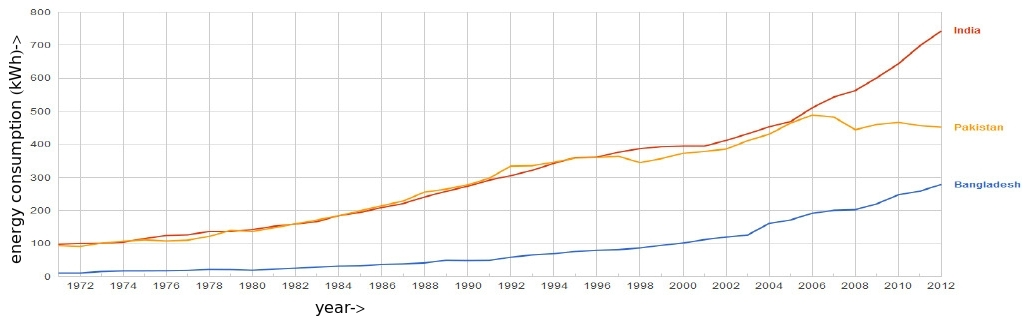
\includegraphics[width=\linewidth]{power_consumption_graph}
		\caption{Statistics of Power Consumption in India (Source: World Bank, 2016) \cite{raghu2017assessing}}
		\label{power_consumption_graph}
	\end{figure}
	\pagenumbering{arabic}
	\clearpage
	\chapter{PROJECT DESCRIPTION AND GOALS}
	\Blindtext
	\chapter{TECHNICAL SPECIFICATIONS}
	\Blindtext
	
	\chapter{DESIGN APPROACH AND DETAILS}
	\section{Design Approach / Materials \& Methods}
	\Blindtext
	\section{Codes and Standards}
	\Blindtext
	\section{Constraints, Alternatives and Tradeoffs}
	\Blindtext
	\chapter{SCHEDULE, TASKS AND MILESTONES}
	\Blindtext
	\lstinputlisting[language=Python]{./codes/samplecode.py}
	\chapter{PROJECT DEMONSTRATION}
	\Blindtext
	\chapter{RESULTS \& DISCUSSION} \label{res}
	\Blindtext
	\chapter{SUMMARY}
	\Blindtext
	\clearpage
	\phantomsection
	\addcontentsline{toc}{chapter}{\protect\numberline {9}REFERENCES}%newly added
	\bibliographystyle{IEEEtran}
	\bibliography{IEEEabrv,capstone_rep_bibliography}
	
	\appendices
	\appendixname
	
	
	\includepdf[height=\textheight,pages=107,offset=0 -4cm,pagecommand=\chapter{Schneider PowerLogic Ion 7650 as Modbus Slave}\label{powerLogic_guide}]{./appendices/ion_user_guide.pdf}
	\includepdf[pages={108-111}]{./appendices/ion_user_guide.pdf}
	
	
	
	
	
	\chapter{Pin Diagram of Raspberry Pi}
	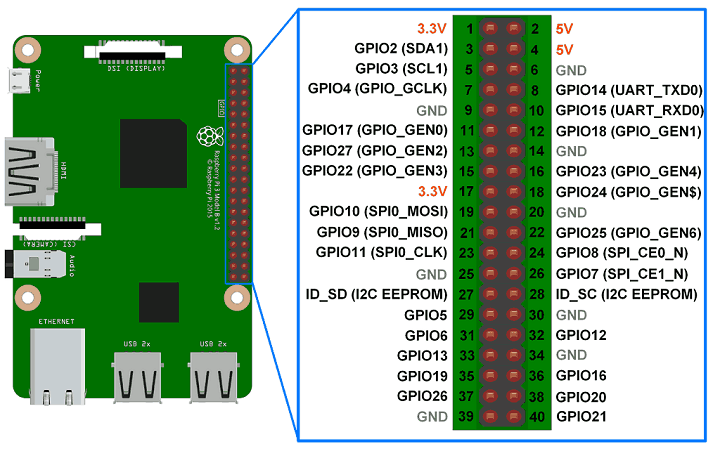
\includegraphics[width=\linewidth]{raspberry_pin_diag}
	
	
	
	
\end{document}
